\documentclass[11pt,oneside,final]{memoir}

\makeatletter
\usepackage{soul}
\usepackage[cmyk]{xcolor}

\usepackage[pdftex]{graphicx}
\graphicspath{{../../images/}}
\usepackage{eso-pic}
\usepackage{calc}

\usepackage{geometry}
\geometry{
paperwidth=135mm,
paperheight=120mm,
nohead,
nofoot,
vmargin=5mm,
hmargin=5mm
}
\setstocksize{120mm}{135mm}

\usepackage{fontspec}
\setmainfont[Ligatures = TeX]{Shaker 2 Light}

\newfontfamily\titleFont[Ligatures = TeX]{Shaker 2 Light}
%\newfontfamily\subtitleFont[Ligatures = TeX]{Shaker 2 Regular}
\newfontfamily\subtitleFont[Ligatures = TeX]{Shaker 2 Light}
\newfontfamily\authorFont[Ligatures = TeX]{Shaker 2 Regular}

\sodef\soTitle{}{.1em}{.5em plus.1em}{.1em plus.1em minus.1em}
\sodef\soAuthor{}{.05em}{.5em plus.1em}{.1em plus.1em minus.1em}

\newcommand\titleSize{\@setfontsize\titleSize{18}{19}}

\pagestyle{empty}

\setlength{\parindent}{0pt}

\newlength\coverImageHeight
% add +1mm to compensate for top-bleed
\setlength\coverImageHeight{63mm}

\newlength\coverImageY
\setlength\coverImageY{\paperheight-\coverImageHeight+1mm}

\newlength\beforeTitleSkip
\setlength\beforeTitleSkip{\coverImageHeight-1mm-5mm+8mm}

\makeatother

\begin{document}

\centering
%\pagecolor[cmyk]{0.45,0.45,0.47,0.06}
%\pagecolor[RGB]{137, 101, 82}

\AddToShipoutPictureFG*{\put(\LenToUnit{-1mm},\LenToUnit{\coverImageY}){
\begin{minipage}[b][\coverImageHeight][b]{\paperwidth + 2mm}%
\centering%
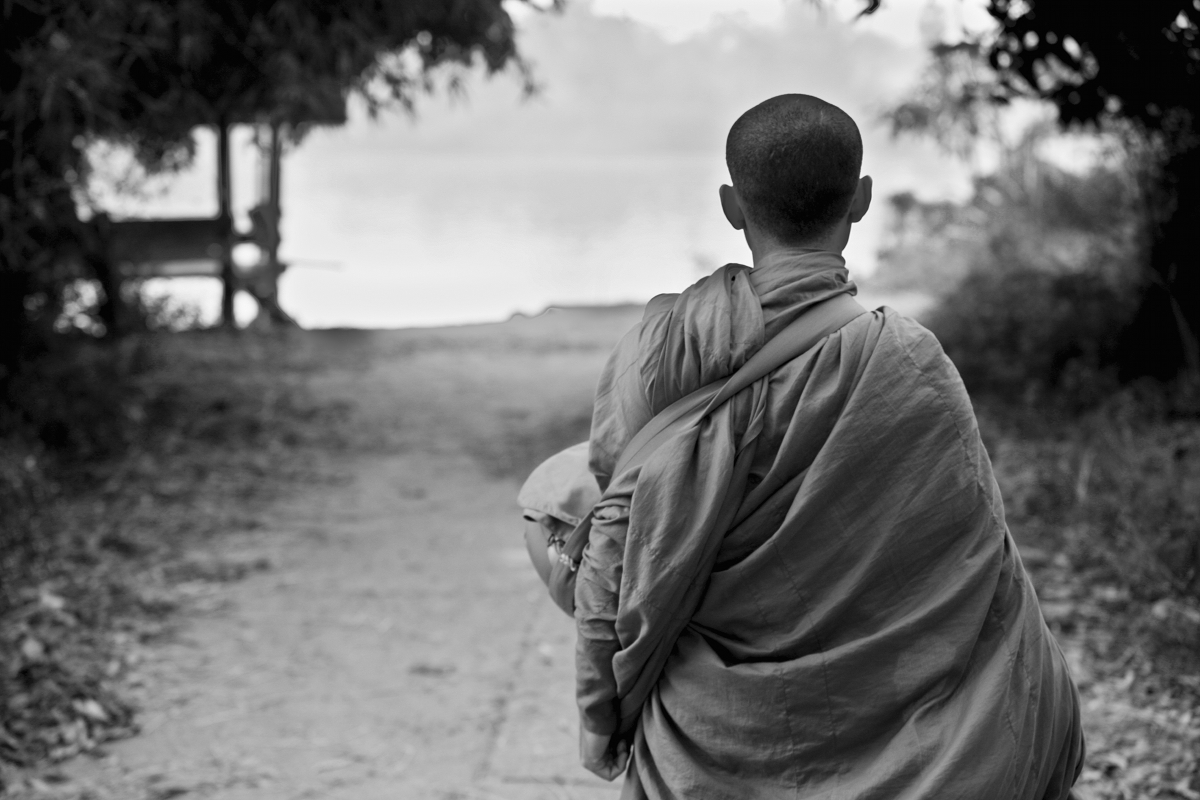
\includegraphics[height=\coverImageHeight,keepaspectratio]
{cover_photo.jpg}%
\end{minipage}%
}}%

\vspace*{\beforeTitleSkip}

{\titleFont\titleSize\color[gray]{0.2}\soTitle{Dhammapada Reflections}}

\vspace*{\baselineskip}

\vfill

{\authorFont\normalsize\color[gray]{0.2}\soAuthor{Ajahn Munindo}}

\vfill

{\raggedleft
\textcolor[gray]{0.5}{Vol. 1}
\par
}

\end{document}
